Interleaving of the stages of multiple jobs is our key concept for enabling large-scale autotuning. \cite{Ma.2005} uses a design-time scheduler to create a program with good concurrency. We need to dynamically schedule incoming jobs, so the schedule cannot be predetermined. We need an additional component in the autotuning architecture that orchestrates running jobs. In this chapter, we describe the design and implementation of our central scheduler that controls stage execution.

\section{Design}
Our scheduler possesses the two features that have been determined to be imperative for optimal large-scale autotuning:
\begin{itemize}
	\item Computation resources are shared between jobs. This facilitates good resource utilization since the idle time of one job can be leveraged to execute another job. This is called \textit{interleaving} and saves hardware and costs as a result. However, stage dependencies of a single job must be maintained.
	\item Interference between jobs is prevented. This guarantees that inference performance and autotuning time are as good as possible. The scheduler needs to check if the resource that will be used by the next stage is free before execution. This might necessitate the postponing of stage executions if the stage is ready before the resource becomes free.
\end{itemize}
These two features not only make it match the optimal solution, but also do they solve the problem of bad resource utilization of single-job autotuning by leveraging that shortcoming.

In case multiple jobs are ready, the scheduler needs to decide which one to run. The simplest approach is to use a round-robin algorithm, which iterates over the jobs in the order they were started and picks the first one that is ready. More sophisticated approaches might apply some logic to decide on a job which would maximize resource utilization but keep the average autotuning time low. However, we choose the round-robin algorithm for our first version. It is easy to implement and works reasonably well for an arbitrary number of jobs, which allows us to proof our concept.

\begin{figure}[h]
	\centering
	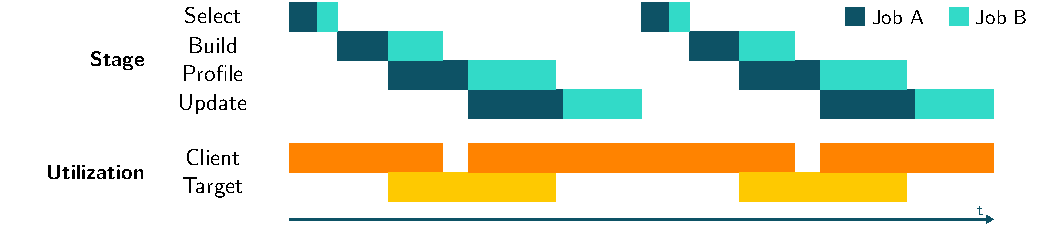
\includegraphics[width=\textwidth]{tvm_resource_utilization_interleaving}%
	\caption{Interleaving of multiple autotuning jobs}
	\label{fig:interleaving}
\end{figure}

Figure \ref{fig:interleaving} illustrates round-robin-based interleaving with an example of two jobs. Significant events are marked with numbers. Job A and Job B are started at the same time, but assume that the scheduler knows first about A. The first stage of A is executed, then the first stage of B. Once B finishes, the round-robin algorithm decides it is A's turn again and executes its second stage. However, a more sophisticated algorithm might have decided that it is better to let B execute first. Once A finishes the seconds stage, the client machine is free and B can execute the second stage. At the same time, A is ready to execute the third stage which will run on the target device. Since the target device is not in use, A can execute the profiling there in parallel to B's building since they use separate resources (\textbf{\textit{1}}). Building does not take as long as profiling, so A is ready to profile before B finishes its profiling stage. Therefore, A's third stage is postponed until the target device is free (\textbf{\textit{2}}). A's profiling and B's update model can, once again, execute simultaneously since they use distinct resources. After one iteration of all four stages, the process starts anew with the first stage (\textbf{\textit{3}}). This continues until both jobs are done. In a real scenario, new jobs might appear while other jobs are already running. The round-robin scheduler simply adds them to its list of jobs and includes them in the interleaving. Note how the resource utilization in Figure \ref{fig:interleaving} is much improved over the single-job autotuning in Figure \ref{fig:tvm-res-util} due to overlapping and sharing. Especially on the client device, utilization has almost been maximized since three of the four stages use the client.

\subsection{Scheduling Algorithm}
to keep scheduler algorithm simple, we designed it to be agnostic of stages
scheduler needs to know
- knows which job will use which resource
- knows which resource is currently available
we call this load-aware
theoretically, could work for any application that supports this interface (e.g. TC?)

allows for variable strategies to compare different designs
show scheduling pseudocode

\subsection{Autotuning Decomposition}
Necessary step before implementation
Show figure
Default TVM:
Procedure is monolithic
Start runner and loop does not stop until its finished
We want to be able to control the execution of individual stages

Decompose monolith into separate units for stages
This allows us to control when which stage is being executed
Necessary for scheduler
Runner does not do anything on its own but waits for commands

\section{Implementation}
Figure with autotuning procedure with scheduler
Since TVM only provides a python interface, we are using python 3.5

since only proof-of-concept, very specific to make it work quickly and non-flexible/fault-tolerant
Leverage SimpleTVM


\subsection{RPC}
We want clients to live in different processes, docker containers, possibly physical servers (why?)
requires RPC infrastructure consisting of scheduler and clients
different from TVM RPC infrastructure
clients register to scheduler
describe endpoints

\subsection{Components}
Show whole stack, denote what happens in scheduler, what happens in runner
Show which communication is in-process and which is RPC
JobManager negotiates between autotuning stages interface and simple scheduler interface, keeps track at position in autotuning
show abstract scheduler and client interface

\subsection{Challenges}
initially wanted to run scheduler and clients in one multi-threaded process without RPC to get results quickly
not possible due to python global interpreter lock

evaluation of design choices takes long because autotuning is a slow process, created MockJob for debugging of scheduler

\section{Autotuning as a Service}
imagine autotuning as a service where users can submit their trained model and receive an optimized version according to SLA
Describe as a service
More sophisticated scheduler, requires moving more autotuning logic from client to scheduler
Make client stateless

Keep trained model and update it every n new entries to skip transfer learning time for every task
Check currently known best configurations and see if SLA is already met before actually starting autotuning
Automatically set up autotuning infrastructure
Split jobs on task and search space level to parallelize more
- make better use of unused resources
- faster autotuning, e.g. for paying customers